\section{TMini\-Ntuple\-Analyzer Class Reference}
\label{classTMiniNtupleAnalyzer}\index{TMiniNtupleAnalyzer@{TMiniNtupleAnalyzer}}
Class for private mini ntuples analysis. continue brief description here.  


{\tt \#include $<$TMini\-Ntuple\-Analyzer.h$>$}

Inheritance diagram for TMini\-Ntuple\-Analyzer:\begin{figure}[H]
\begin{center}
\leavevmode
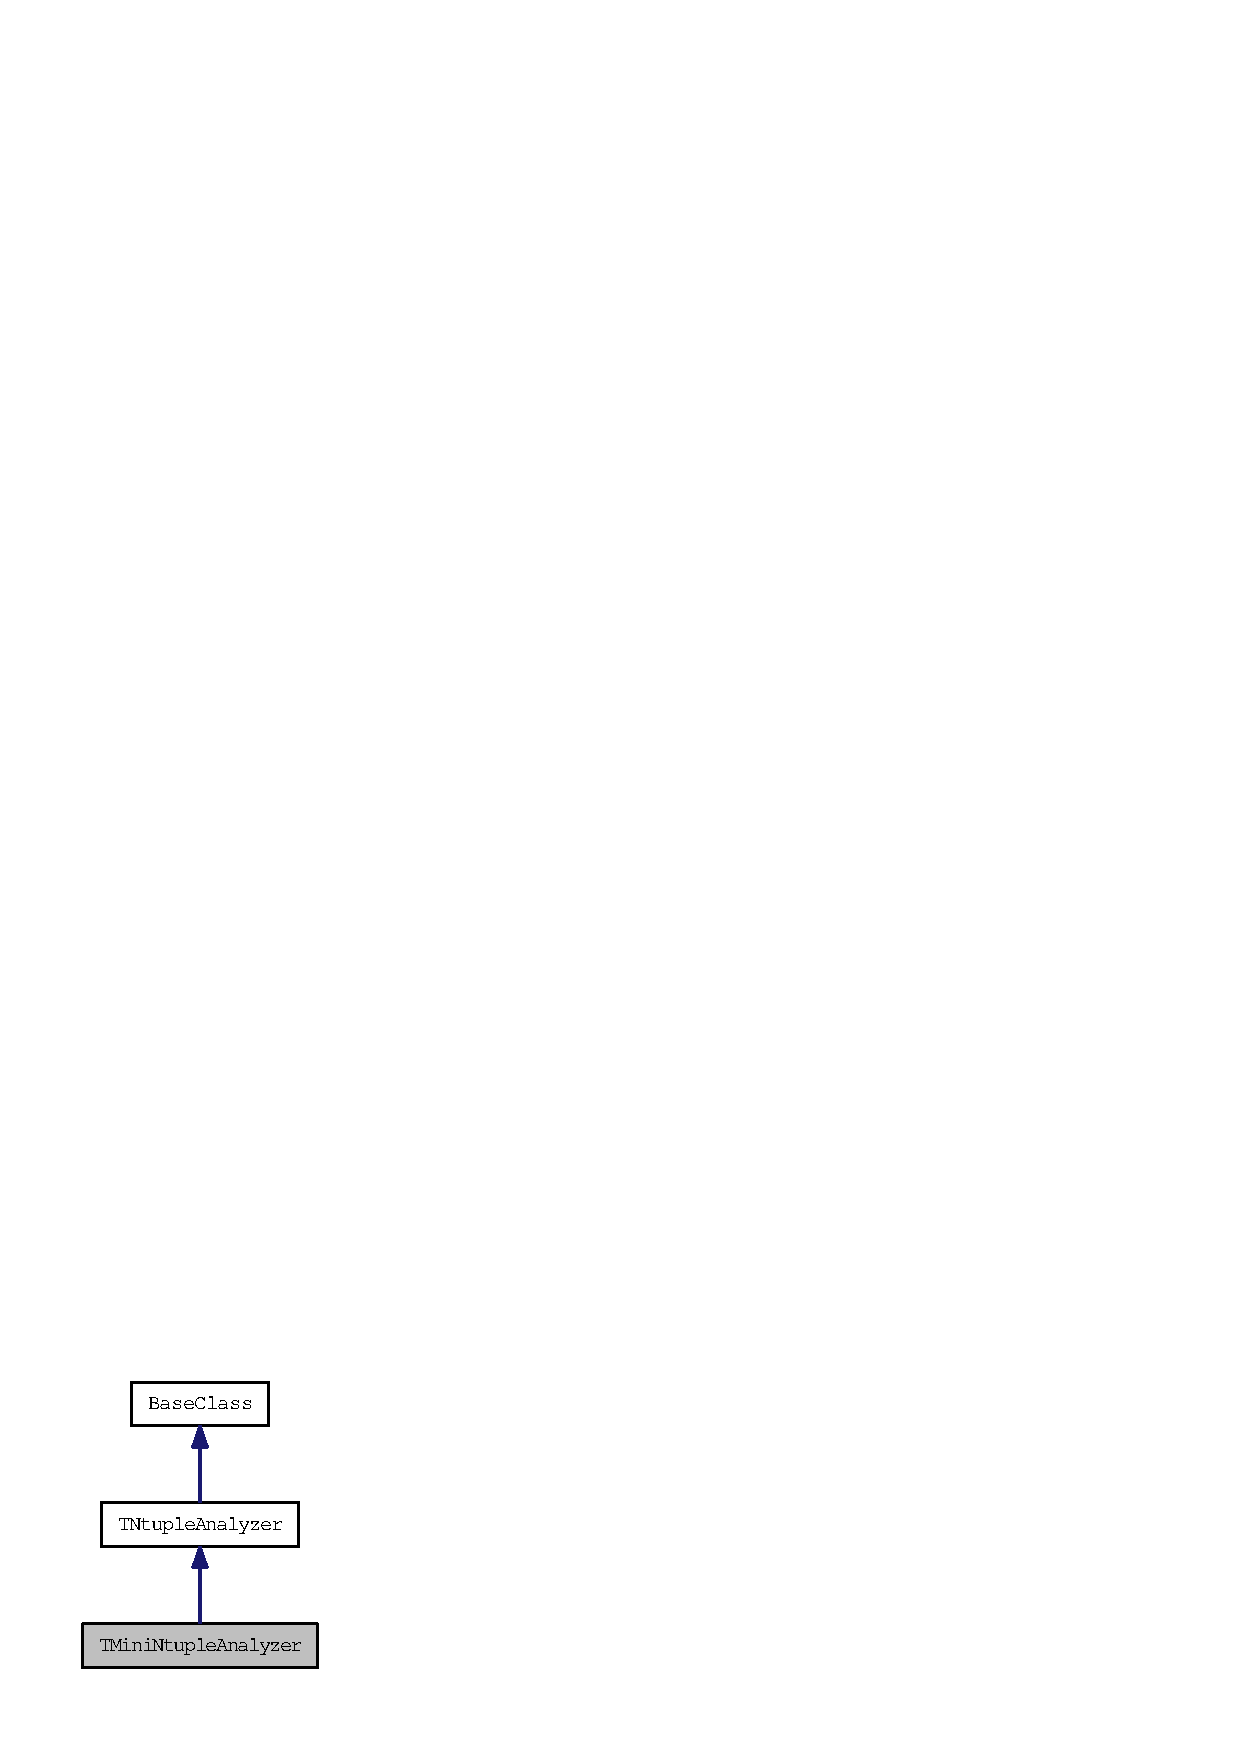
\includegraphics[width=78pt]{classTMiniNtupleAnalyzer__inherit__graph}
\end{center}
\end{figure}
Collaboration diagram for TMini\-Ntuple\-Analyzer:\begin{figure}[H]
\begin{center}
\leavevmode
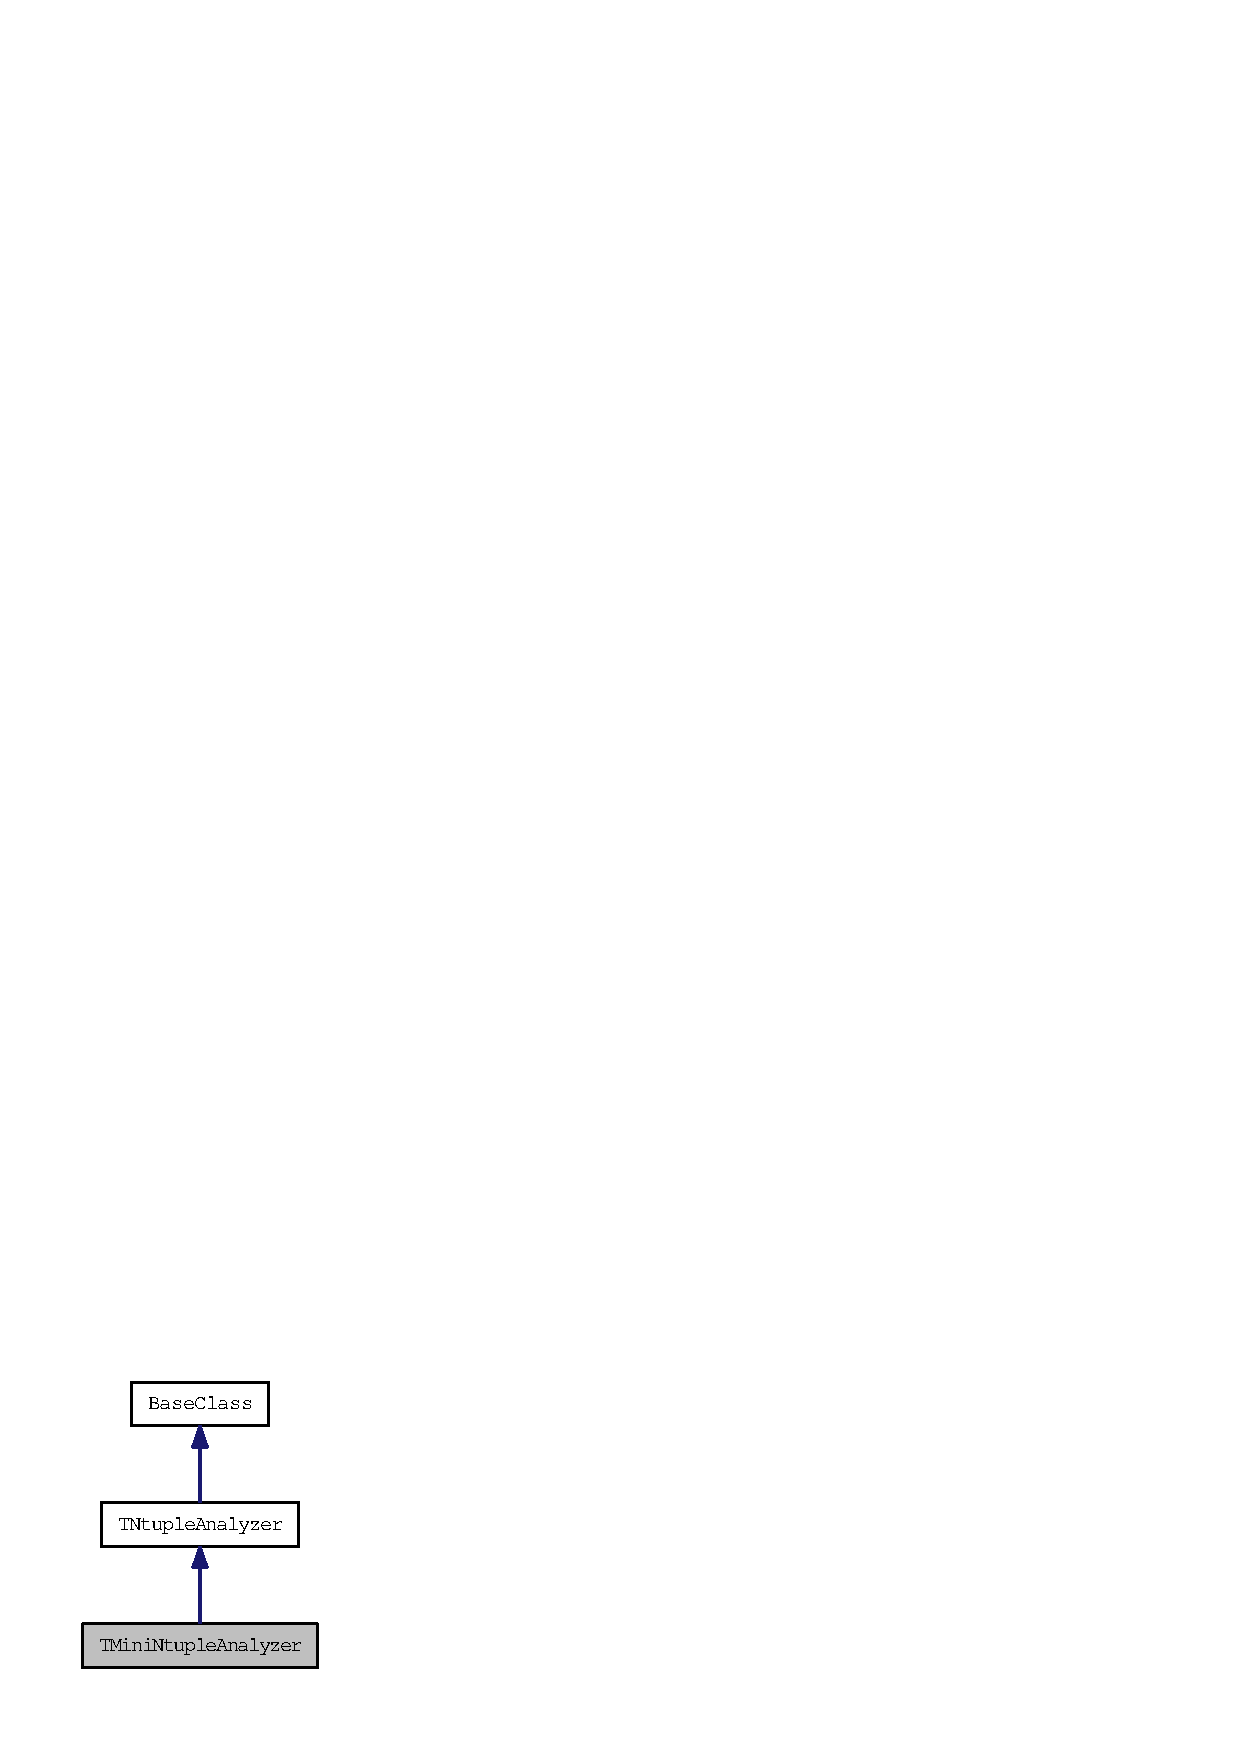
\includegraphics[width=78pt]{classTMiniNtupleAnalyzer__coll__graph}
\end{center}
\end{figure}
\subsection*{Public Member Functions}
\begin{CompactItemize}
\item 
\textbf{TMini\-Ntuple\-Analyzer} (TString Histo\-Version, TString Binning\-File, TString Declare\-Histo\-File\-Name)\label{classTMiniNtupleAnalyzer_1ede6ceb99c7ffc81598e30dae9e321f}

\item 
void \textbf{Set\-Binning\-File\-Name} (TString filename)\label{classTMiniNtupleAnalyzer_096390422b311dbbce27c1de8827d69a}

\item 
void \textbf{Set\-Drop\-Tracks} (bool drop\_\-tracks)\label{classTMiniNtupleAnalyzer_ee46501e8f2958b4873ae723448525c6}

\item 
void \textbf{Set\-Only\-Calculate\-Events\-Per\-Run} (bool calc\_\-events)\label{classTMiniNtupleAnalyzer_ba5919ba7d3a0bfc5926a31a29833776}

\item 
void \textbf{Set\-Secondary\-Vertex\-Smearing} (bool smear)\label{classTMiniNtupleAnalyzer_e58b5e858e9177ea39f723d35ee5c8f4}

\item 
void \textbf{Set\-Drop\-Track\-Probability} (Float\_\-t prob)\label{classTMiniNtupleAnalyzer_a8302ceb976cf37bab9aa2071bb6c17e}

\item 
void \textbf{Set\-Et\-Reweighting\-LF\_\-filename} (TString name)\label{classTMiniNtupleAnalyzer_55dd3d0f87f8cf8dc7bf3b9330579d37}

\item 
void \textbf{Set\-Et\-Reweighting\-LF} (bool do\_\-reweighting)\label{classTMiniNtupleAnalyzer_d18515e2a69a3297f7d52b27c0892e96}

\item 
void \textbf{Set\-Test\-First\-Event} (unsigned first\_\-event)\label{classTMiniNtupleAnalyzer_31702ea04ef8454a7db0facef9796c8c}

\item 
void \textbf{Set\-Seed\-Vertex\-Smearing} (unsigned seed1, unsigned seed2)\label{classTMiniNtupleAnalyzer_aa1d0572de17d29a39ef04b3b2db1475}

\item 
void \textbf{Set\-Seed\-Crude\-Tracking\-Efficiency} (unsigned seed)\label{classTMiniNtupleAnalyzer_7cbfe4c310a68720faebb63512e7934a}

\item 
void \textbf{Set\-Jet\-Energy\-Uncertainty} (Double\_\-t jet\_\-unc)\label{classTMiniNtupleAnalyzer_93cc807288017cbbc21426f194af00d0}

\item 
void \textbf{Set\-Vary\-Total\-Jet\-Energy} (bool vary\_\-total)\label{classTMiniNtupleAnalyzer_6a6aba95f0df2e6bd90cc297df38cba7}

\item 
void \textbf{Set\-True\-Level\-Studies} (bool true\_\-studies)\label{classTMiniNtupleAnalyzer_6969912103555ef6e2fabbfffd3f11b7}

\item 
void \textbf{Set\-Fragmentation\-Reweighting\_\-filename} (TString name)\label{classTMiniNtupleAnalyzer_2e860e5d4a99dbd2a7bb3f54e6d69ad8}

\item 
void \textbf{Set\-Fragmentation\-Reweighting} (bool do\_\-reweighting)\label{classTMiniNtupleAnalyzer_2e9486b40352e4028efc8b748127a761}

\item 
void \textbf{Set\-Charm\-Fragmentation\-Reweighting\-Size} (Double\_\-t size)\label{classTMiniNtupleAnalyzer_89dff5653ce3d5c7758610cb8e212c8e}

\item 
void \textbf{Set\-Beauty\-Fragmentation\-Reweighting\-Size} (Double\_\-t size)\label{classTMiniNtupleAnalyzer_a3c6811689465feed0d56189a8d5fdce}

\item 
void \textbf{Set\-Sashas\-Reweighting} (bool apply\_\-reweighting)\label{classTMiniNtupleAnalyzer_f5d84f6d73304e673fd552217f754572}

\item 
void \textbf{Set\-Jet\-Et\-Cut} (Double\_\-t jet\_\-et\_\-cut)\label{classTMiniNtupleAnalyzer_4279e3fdf8fb6c409354c2cc725e9eb1}

\item 
void \textbf{Initialize} ()\label{classTMiniNtupleAnalyzer_f45fbaeab2c8ac85850ebe02cf4aaa61}

\item 
void \textbf{Recalculate\-Luminosity} ()\label{classTMiniNtupleAnalyzer_87ec4b8d4497b61f823dc25d83caa1ab}

\item 
void \bf{Loop} (Bool\_\-t Is\-Inclusive)
\item 
void \textbf{Loop\_\-v04b} (Bool\_\-t Is\-Inclusive)\label{classTMiniNtupleAnalyzer_d226b43fbd71635668eb39a8646265a4}

\item 
void \textbf{Print\-Events\-Per\-Run} ()\label{classTMiniNtupleAnalyzer_47e828451d45c38d0868282b36e82ff2}

\item 
void \textbf{Set\-Printing\-Freq} (Int\_\-t events)\label{classTMiniNtupleAnalyzer_0f54ab2aa775179b9701ef8e7046775f}

\item 
void \textbf{Set\-Rund\-Cache} (bool run\_\-dcache)\label{classTMiniNtupleAnalyzer_b4c91f3788b04947d5722abb92fcaeff}

\item 
void \textbf{Set\-Do\-Jet\-Energy\-Scale\-Syst} (bool do\_\-syst)\label{classTMiniNtupleAnalyzer_e22f4d3617f21f45717d536393ae7d1d}

\item 
void \textbf{Set\-Redo\-Vertexing} (bool redo\_\-vertexing)\label{classTMiniNtupleAnalyzer_9dc051f8b05d12c4df23ba0d9fa01c09}

\item 
void \textbf{Set\-Rcut} (Float\_\-t r\_\-cut)\label{classTMiniNtupleAnalyzer_453f96bcd8c697328469551328401822}

\item 
void \bf{Setp\-T} (Float\_\-t pt\_\-cut)\label{classTMiniNtupleAnalyzer_8e067f95b28cb586b46de02b30359fd2}

\begin{CompactList}\small\item\em Set Cone cut. \item\end{CompactList}\item 
void \bf{Set\-STT} (Int\_\-t stt)\label{classTMiniNtupleAnalyzer_a00d97542e694747983ccfda316c58ed}

\begin{CompactList}\small\item\em Set minimal track p\-T. \item\end{CompactList}\item 
void \bf{Set\-CTD} (Int\_\-t ctd)\label{classTMiniNtupleAnalyzer_8861900ad6c57f4014d621c9a6b4e67e}

\begin{CompactList}\small\item\em Set minimal number of STT hits. \item\end{CompactList}\item 
void \bf{Set\-MVD} (Int\_\-t mvd)\label{classTMiniNtupleAnalyzer_ba084ef27cc6aa3d203ba9b4329901d1}

\begin{CompactList}\small\item\em Set minimal number of CTD hits. \item\end{CompactList}\item 
void \bf{Set\-Use\-Helix\-Track\-Parameters} (Bool\_\-t set\-Helix)\label{classTMiniNtupleAnalyzer_8928626bfe9fc2698193cc248f4a4149}

\begin{CompactList}\small\item\em Set minimal number of MVD hits. \item\end{CompactList}\end{CompactItemize}
\subsection*{Public Attributes}
\begin{CompactItemize}
\item 
Bool\_\-t \textbf{f\-Secondary\-Vertex\-Found}\label{classTMiniNtupleAnalyzer_46ae045134fe9b4cbe4514ddd10e6b66}

\item 
Float\_\-t \textbf{f\-Significance}\label{classTMiniNtupleAnalyzer_cf32c85386178f9363dd0a751f9c466c}

\item 
Float\_\-t \textbf{f\-Reco\-Jet\-Et}\label{classTMiniNtupleAnalyzer_054406aad66adb1ce8d1d5f3b2227320}

\item 
Float\_\-t \textbf{f\-Reco\-Jet\-Eta}\label{classTMiniNtupleAnalyzer_6d0d4038506ecb42d284b8494a62eea0}

\item 
Float\_\-t \textbf{f\-Reco\-Jet\-Phi}\label{classTMiniNtupleAnalyzer_6fff0c7817b2a718c949d0480492f379}

\item 
Float\_\-t \textbf{f\-True\-Jet\-Et}\label{classTMiniNtupleAnalyzer_9aa6463690353e13395ba2711a4f38cc}

\item 
Float\_\-t \textbf{f\-True\-Jet\-Eta}\label{classTMiniNtupleAnalyzer_920e554d9b1dc193b535b0f19a9445b3}

\item 
Float\_\-t \textbf{f\-True\-Jet\-Phi}\label{classTMiniNtupleAnalyzer_1520727f726cd765e73256caaeffe91d}

\item 
Bool\_\-t \textbf{f\-Fill\-Mirrored}\label{classTMiniNtupleAnalyzer_6b52adfde82d38de9743201443b74652}

\item 
vector$<$ \bf{TVertex} $>$ \textbf{f\-Vertices}\label{classTMiniNtupleAnalyzer_88081b1374178f61a78f859ac28e181d}

\item 
vector$<$ \bf{TVertex} $>$ \textbf{f\-Vertices\-Refitted}\label{classTMiniNtupleAnalyzer_fd83d2a460c9b26e048231631f8bfcaf}

\item 
Float\_\-t \textbf{f\-True\_\-y}\label{classTMiniNtupleAnalyzer_7fd18e588f63ac92979f031cf7d4531f}

\item 
Bool\_\-t \textbf{f\-Apply\-Smearing}\label{classTMiniNtupleAnalyzer_9e941561cceb58648b37655a43643a1f}

\item 
Double\_\-t \textbf{f\-Smearing\-Gauss1Prob}\label{classTMiniNtupleAnalyzer_c2f43f09648864a5b51155e963d39ab8}

\item 
Double\_\-t \textbf{f\-Smearing\-Gauss1Width}\label{classTMiniNtupleAnalyzer_dc2b542be84934ab1a0ba4700a1af7b5}

\item 
Double\_\-t \textbf{f\-Smearing\-Gauss2Prob}\label{classTMiniNtupleAnalyzer_3510a75b60ab335bf397c6a526e35950}

\item 
Double\_\-t \textbf{f\-Smearing\-Gauss2Width}\label{classTMiniNtupleAnalyzer_cfea921ba15de39c42dda8a7c603f2eb}

\item 
Double\_\-t \textbf{f\-Smearing\-Exp\-Prob}\label{classTMiniNtupleAnalyzer_b06fe90699a58728793e4099daef7cea}

\item 
Double\_\-t \textbf{f\-Smearing\-Exp\-Coeff}\label{classTMiniNtupleAnalyzer_931f93158be90e8eefb1a45945510e32}

\item 
Bool\_\-t \textbf{f\-True\-Level\-Studies}\label{classTMiniNtupleAnalyzer_163b0c21dcf6ce3305afdf87d5f7c44d}

\end{CompactItemize}
\subsection*{Private Member Functions}
\begin{CompactItemize}
\item 
void \bf{Set\-Binning} ()
\item 
void \textbf{Calculate\-Charm\-Qg4Weighting\-Factor} ()\label{classTMiniNtupleAnalyzer_c92d7e494caf54acbba8a37f5f10d339}

\item 
void \textbf{Initialize\-Random\-Generators} ()\label{classTMiniNtupleAnalyzer_3126fced39cf3c5ffacc8147b9718a0f}

\item 
void \textbf{Create\-Bin\-Histograms} ()\label{classTMiniNtupleAnalyzer_b15d9a6b4809fe1656cd15aaf8c24074}

\item 
void \textbf{Declare\-Histograms} (\bf{TGlobal\-Bin} $\ast$tgb)\label{classTMiniNtupleAnalyzer_68e2ab7e18207f888db945789dab9143}

\item 
void \textbf{Fill\-Hist} (\bf{TGlobal\-Bin} $\ast$tgb, TString Hist\-Title, Float\_\-t Value)\label{classTMiniNtupleAnalyzer_d078c6a6a7fcb59db823bd1ce0e66a8d}

\item 
void \textbf{Mirror\-Histogram\-OLD} (TString Hist\-Name)\label{classTMiniNtupleAnalyzer_f9cc0e8c6569b4537dcd1e6d4b7d5769}

\item 
void \textbf{Mirror\-Histograms} ()\label{classTMiniNtupleAnalyzer_ded815e11411ec9addbf9a0513fcbf1b}

\item 
Float\_\-t \bf{Calculate\-Significance} (Int\_\-t vertex)
\item 
Float\_\-t \textbf{Calculate\-Proj\-Decay\-Length} (Int\_\-t vertex)\label{classTMiniNtupleAnalyzer_a87777b9eb8adcf55ad51df1a2f59fad}

\item 
Bool\_\-t \bf{Is\-DIS} ()
\item 
void \textbf{Write\-Histograms} ()\label{classTMiniNtupleAnalyzer_970b02310941a636c1a14dd130c789fa}

\item 
void \textbf{Get\-Et\-Reweighting\-LF\_\-histo} ()\label{classTMiniNtupleAnalyzer_2847a69f60c3518fb426f3b581bbded8}

\item 
Float\_\-t \textbf{get\-Et\-Reweighting} (Float\_\-t jet\_\-et)\label{classTMiniNtupleAnalyzer_33db0be8a39f9f9e605810559ae31c68}

\item 
void \textbf{Get\-Fragmentation\-Reweighting\_\-Histo} ()\label{classTMiniNtupleAnalyzer_f4a790d3344bdb1d38aae5d560cdacea}

\item 
Int\_\-t \textbf{get\-Reweighting\-Histo\-Bin} (TH1F $\ast$histo, Float\_\-t value)\label{classTMiniNtupleAnalyzer_6e37dcd6ef5935c1070159912c6579a1}

\item 
void \bf{find\-Vertices} ()
\end{CompactItemize}
\subsection*{Private Attributes}
\begin{CompactItemize}
\item 
bool \textbf{f\-Run\_\-d\-Cache}\label{classTMiniNtupleAnalyzer_6f81e43a548bc42e88b97ba89e3b2ea4}

\item 
TFile $\ast$ \textbf{f\-Histograms\-File}\label{classTMiniNtupleAnalyzer_7117078c305fc5aeb484503408fce4d8}

\item 
TString \textbf{f\-Histograms\-File\-Version}\label{classTMiniNtupleAnalyzer_203a35b01f771f192be44cb7255d95f9}

\item 
TList $\ast$ \textbf{f\-List\_\-TGlobal\-Bin}\label{classTMiniNtupleAnalyzer_ab102b41f9e4f98a97b7a23e44098ad4}

\item 
TH1F $\ast$ \textbf{f\-Debug\-SVTX}\label{classTMiniNtupleAnalyzer_88182d7246cb4a9f90e0a21b027ac757}

\item 
TString \textbf{f\-Binning\-File\-Name}\label{classTMiniNtupleAnalyzer_4fb9778772f4b02397900313981398ff}

\item 
TString \textbf{f\-Histogram\-Declaration\-File}\label{classTMiniNtupleAnalyzer_cf1dbe9a923f244a20f259a65ca5c58c}

\item 
Bool\_\-t \textbf{f\-Apply\-Q2g4Weighting}\label{classTMiniNtupleAnalyzer_3333cca9f37c521d8a469fce22ef62a9}

\item 
Double\_\-t \textbf{f\-Charm\-Q2g4Weight}\label{classTMiniNtupleAnalyzer_597247d64ebd4e2c250adbeaa61a0204}

\item 
Double\_\-t \textbf{f\-True\-Q2Weight}\label{classTMiniNtupleAnalyzer_828cc55ebbe3891d6efbcbbefbf7487f}

\item 
Double\_\-t \textbf{f\-Reco\-Q2Weight}\label{classTMiniNtupleAnalyzer_9f3b6565489bb61f939c0c2452c256e6}

\item 
TRandom3 $\ast$ \textbf{rnd}\label{classTMiniNtupleAnalyzer_0bc634b7c6811ebed6e7575488ff2c4a}

\item 
TRandom3 $\ast$ \textbf{rnd2}\label{classTMiniNtupleAnalyzer_c3bda989da04d86057b764a6a23a4339}

\item 
TRandom3 $\ast$ \textbf{rnd\_\-eff}\label{classTMiniNtupleAnalyzer_c663e958b428a3e7fc82574556ac4410}

\item 
unsigned \textbf{f\-Seed\_\-rnd}\label{classTMiniNtupleAnalyzer_157ce77acdb78e89b5b624997953dbed}

\item 
unsigned \textbf{f\-Seed\_\-rnd2}\label{classTMiniNtupleAnalyzer_895545cc133bc8a25fc9ecd075dc8f82}

\item 
unsigned \textbf{f\-Seed\_\-rnd\_\-eff}\label{classTMiniNtupleAnalyzer_a3a15d4f1a7dab0b2d6e15ae44e0c39c}

\item 
bool \textbf{f\-Drop\-Tracks}\label{classTMiniNtupleAnalyzer_a3bb463a80509166638e0fbd7ad44a4e}

\item 
Float\_\-t \textbf{f\-Drop\-Probability}\label{classTMiniNtupleAnalyzer_45954a7e9516b124d3810381bc0a6cd5}

\item 
std::map$<$ unsigned, unsigned $>$ \textbf{f\-Events\-Per\-Run\_\-ALL}\label{classTMiniNtupleAnalyzer_4ad69c6cee3e08c3a9af9a68f2bdcec4}

\item 
std::map$<$ unsigned, unsigned $>$ \textbf{f\-Events\-Per\-Run\_\-EVTAKE\_\-MVDTAKE}\label{classTMiniNtupleAnalyzer_3cc76aa4175012565fe3eecd2c892717}

\item 
bool \textbf{f\-Only\-Calculate\-Events\-Per\-Run}\label{classTMiniNtupleAnalyzer_62fa5db0fa71ff8e84215b2e673d4b35}

\item 
TH1F $\ast$ \textbf{f\-Et\-Reweighting\-LF\_\-histo}\label{classTMiniNtupleAnalyzer_f800389e731788a3e81526879b6d9443}

\item 
TString \textbf{f\-Et\-Reweighting\-LF\_\-filename}\label{classTMiniNtupleAnalyzer_4df3a9b546c3fc0bf3ff40c92db308c1}

\item 
bool \textbf{f\-Et\-Reweighting\-LF}\label{classTMiniNtupleAnalyzer_88b17291ea3e29036cb98355e95f9367}

\item 
TH1F $\ast$ \textbf{f\-Fragmentation\-Reweighting\_\-histo}\label{classTMiniNtupleAnalyzer_6b10478218a36e623c128e762fa12e5a}

\item 
TString \textbf{f\-Fragmentation\-Reweighting\_\-filename}\label{classTMiniNtupleAnalyzer_6e542be9d424791b1d8f93def6a0d1ab}

\item 
bool \textbf{f\-Fragmentation\-Reweighting}\label{classTMiniNtupleAnalyzer_158ba453394546d21ee11acf23dcc8f2}

\item 
unsigned \textbf{f\-Test\-First\-Event}\label{classTMiniNtupleAnalyzer_0faf703ce06c4057304e5beacf762144}

\item 
Double\_\-t \textbf{f\-Jet\-Energy\-Uncertainty}\label{classTMiniNtupleAnalyzer_6a2598b23f4bb4b704741fa5596359dd}

\item 
bool \textbf{f\-Vary\-Total\-Jet\-Energy}\label{classTMiniNtupleAnalyzer_9c852570c432f662cfb7399e1771fdaa}

\item 
bool \textbf{f\-Do\-Jet\-Energy\-Scale\-Syst}\label{classTMiniNtupleAnalyzer_2e328562364b737ae244a6eb6e0fc64e}

\item 
Double\_\-t \textbf{f\-Zstring\_\-weight}\label{classTMiniNtupleAnalyzer_fb1fac10110a18a450c5c4cb08c17250}

\item 
Double\_\-t \textbf{f\-Charm\-Fragm\_\-variation\_\-size}\label{classTMiniNtupleAnalyzer_b031b35499cbe98b211b1c26cc6ea7a3}

\item 
Double\_\-t \textbf{f\-Beauty\-Fragm\_\-variation\_\-size}\label{classTMiniNtupleAnalyzer_b9a5c977389baba4f9d6530a92191703}

\item 
Bool\_\-t \textbf{f\-Sashas\-Reweighting}\label{classTMiniNtupleAnalyzer_371adf0ee3036de1cee6e26680cb51c8}

\item 
Double\_\-t \textbf{f\-Jet\-Et\-Cut}\label{classTMiniNtupleAnalyzer_b02d3cdae79641d27837cbf7f873610b}

\item 
Int\_\-t \textbf{f\-Printing\-Freq}\label{classTMiniNtupleAnalyzer_abf29c3a66d01e502fe9309b689a746a}

\item 
Bool\_\-t \bf{f\-Redo\-Vertexing}\label{classTMiniNtupleAnalyzer_cb7a2e8894285eda92d069480d80a58b}

\begin{CompactList}\small\item\em redo secondary vertexing (including track selection) on the CN level \item\end{CompactList}\item 
Float\_\-t \bf{f\-Rcut}\label{classTMiniNtupleAnalyzer_c464056b6252849618ac0de519f0cf73}

\begin{CompactList}\small\item\em Cone cut. \item\end{CompactList}\item 
Float\_\-t \bf{fp\-T}\label{classTMiniNtupleAnalyzer_6f9774ed3f9991032746042e57a616bd}

\begin{CompactList}\small\item\em minimal track p\-T \item\end{CompactList}\item 
Int\_\-t \bf{f\-STT}\label{classTMiniNtupleAnalyzer_124e5bb0ca6cbd356d9d335ed5722a35}

\begin{CompactList}\small\item\em minimal number of STT hits \item\end{CompactList}\item 
Int\_\-t \bf{f\-CTD}\label{classTMiniNtupleAnalyzer_958ea86244f6d80df4bb39f575a892cf}

\begin{CompactList}\small\item\em OR minimal number of CTD hits. \item\end{CompactList}\item 
Int\_\-t \bf{f\-MVD}\label{classTMiniNtupleAnalyzer_a21747d03ef6eea83319922a9c221fe0}

\begin{CompactList}\small\item\em minimal number of MVD hits \item\end{CompactList}\item 
Bool\_\-t \bf{f\-Use\-Helix\-Track\-Parameters}\label{classTMiniNtupleAnalyzer_b45bcc3aa0973e98679a79e1c07d0bdc}

\begin{CompactList}\small\item\em whether to use Trk\_\-Helix or Tracking \item\end{CompactList}\end{CompactItemize}


\subsection{Detailed Description}
Class for private mini ntuples analysis. continue brief description here. 

put detailed description here 



\subsection{Member Function Documentation}
\index{TMiniNtupleAnalyzer@{TMini\-Ntuple\-Analyzer}!CalculateSignificance@{CalculateSignificance}}
\index{CalculateSignificance@{CalculateSignificance}!TMiniNtupleAnalyzer@{TMini\-Ntuple\-Analyzer}}
\subsubsection{\setlength{\rightskip}{0pt plus 5cm}Float\_\-t TMini\-Ntuple\-Analyzer::Calculate\-Significance (Int\_\-t {\em vertex})\hspace{0.3cm}{\tt  [private]}}\label{classTMiniNtupleAnalyzer_a7537fd25023e3b2532e94a1b36e6ef4}


\index{TMiniNtupleAnalyzer@{TMini\-Ntuple\-Analyzer}!findVertices@{findVertices}}
\index{findVertices@{findVertices}!TMiniNtupleAnalyzer@{TMini\-Ntuple\-Analyzer}}
\subsubsection{\setlength{\rightskip}{0pt plus 5cm}void TMini\-Ntuple\-Analyzer::find\-Vertices ()\hspace{0.3cm}{\tt  [private]}}\label{classTMiniNtupleAnalyzer_1594ee453f064ac321029c75db916487}


replacement for orange sec vtx finder - to allow more flexibility like lower track p\-T cut \index{TMiniNtupleAnalyzer@{TMini\-Ntuple\-Analyzer}!IsDIS@{IsDIS}}
\index{IsDIS@{IsDIS}!TMiniNtupleAnalyzer@{TMini\-Ntuple\-Analyzer}}
\subsubsection{\setlength{\rightskip}{0pt plus 5cm}Bool\_\-t TMini\-Ntuple\-Analyzer::Is\-DIS ()\hspace{0.3cm}{\tt  [private]}}\label{classTMiniNtupleAnalyzer_ba8ec5add8c28d9d120c2b68dbf6557a}


\index{TMiniNtupleAnalyzer@{TMini\-Ntuple\-Analyzer}!Loop@{Loop}}
\index{Loop@{Loop}!TMiniNtupleAnalyzer@{TMini\-Ntuple\-Analyzer}}
\subsubsection{\setlength{\rightskip}{0pt plus 5cm}void TMini\-Ntuple\-Analyzer::Loop (Bool\_\-t {\em Is\-Inclusive})}\label{classTMiniNtupleAnalyzer_15caaf33cb18e1a0b229e37907958896}


\index{TMiniNtupleAnalyzer@{TMini\-Ntuple\-Analyzer}!SetBinning@{SetBinning}}
\index{SetBinning@{SetBinning}!TMiniNtupleAnalyzer@{TMini\-Ntuple\-Analyzer}}
\subsubsection{\setlength{\rightskip}{0pt plus 5cm}void TMini\-Ntuple\-Analyzer::Set\-Binning ()\hspace{0.3cm}{\tt  [private]}}\label{classTMiniNtupleAnalyzer_00af1592754549584f500cb9a6ace31e}


Sets binning for analysis. Each bin is processed in the same way. 

choose your binning here, use: TGlobal\-Bin::Add\-Bin(pointer to TBin) TBin::TBin(descripiton of the variable, ptr to it,lower\-Limit, upper\-Limit) don't forget to add them to f\-List\_\-TGlobal\-Bin at the end of this method Last argument (Variable\-Phase) DETERMINES POINT (Phase) where this variable is checked; Depends on your desing, be careful!!!

Define mapping: variable ID (TString) --$>$ pointyer to the relevant variable. Found no better way than doing it like this.

Read config file with binning definition 

The documentation for this class was generated from the following files:\begin{CompactItemize}
\item 
Ntuple\-Analyzer/inc/TMini\-Ntuple\-Analyzer.h\item 
Ntuple\-Analyzer/src/TMini\-Ntuple\-Analyzer.cxx\item 
Ntuple\-Analyzer/src/TMini\-Ntuple\-Analyzer\-Loop.cxx\item 
Ntuple\-Analyzer/src/TMini\-Ntuple\-Analyzer\-Set\-Binning.cxx\end{CompactItemize}
